\documentclass[a4paper,11pt,oneside]{article}

\usepackage{graphicx}
\usepackage{url}
\usepackage{subfigure}
\usepackage{rotating}
\usepackage[small,bf]{caption}
\usepackage[top=3cm, bottom=3cm, left=3cm, right=3cm]{geometry}

\begin{document}
\author{Richard M. Leggett\\richard.leggett@tgac.ac.uk}
\title{MetaCortex}
\date{\today}
\maketitle

%=========================================================================
\section{Introduction}

MetaCortex is an assembler for metagenomic, or environmental, sequence data. It is based on the consensus version of the Cortex assembler (cortex\_con) developed by Mario Caccamo and Zamin Iqbal \cite{iqbal2012}.
 
%=========================================================================
\section{Key concepts}

%-------------------------------------------------------------------------
\subsection{CTX files}

Though it is possible to go straight from FASTA or FASTQ files to a complete meta-assembly, MetaCortex (like Cortex) implements an intermediate binary file format which enables the parallelisation of the process of converting raw reads into a de Bruijn graph structure. As well as speeding up the overall assembly process by sharing out the reads across multiple processing cores, the approach also makes it possible to carry out big assemblies in lower memory environments.

Figure \ref{fig:typicalprocess} illustrates the typical approach taken with MetaCortex. Reads are separated into files - either by hand, or most likely, because the sequencing instrument has produced multiple files. MetaCortex is then executed in two stages - firstly, in parallel, to import each read file, create a de Bruijn graph of kmers and output a CTX file; then secondly, to combine the separate CTX files and output contigs.

\begin{figure}[tb]
\centering
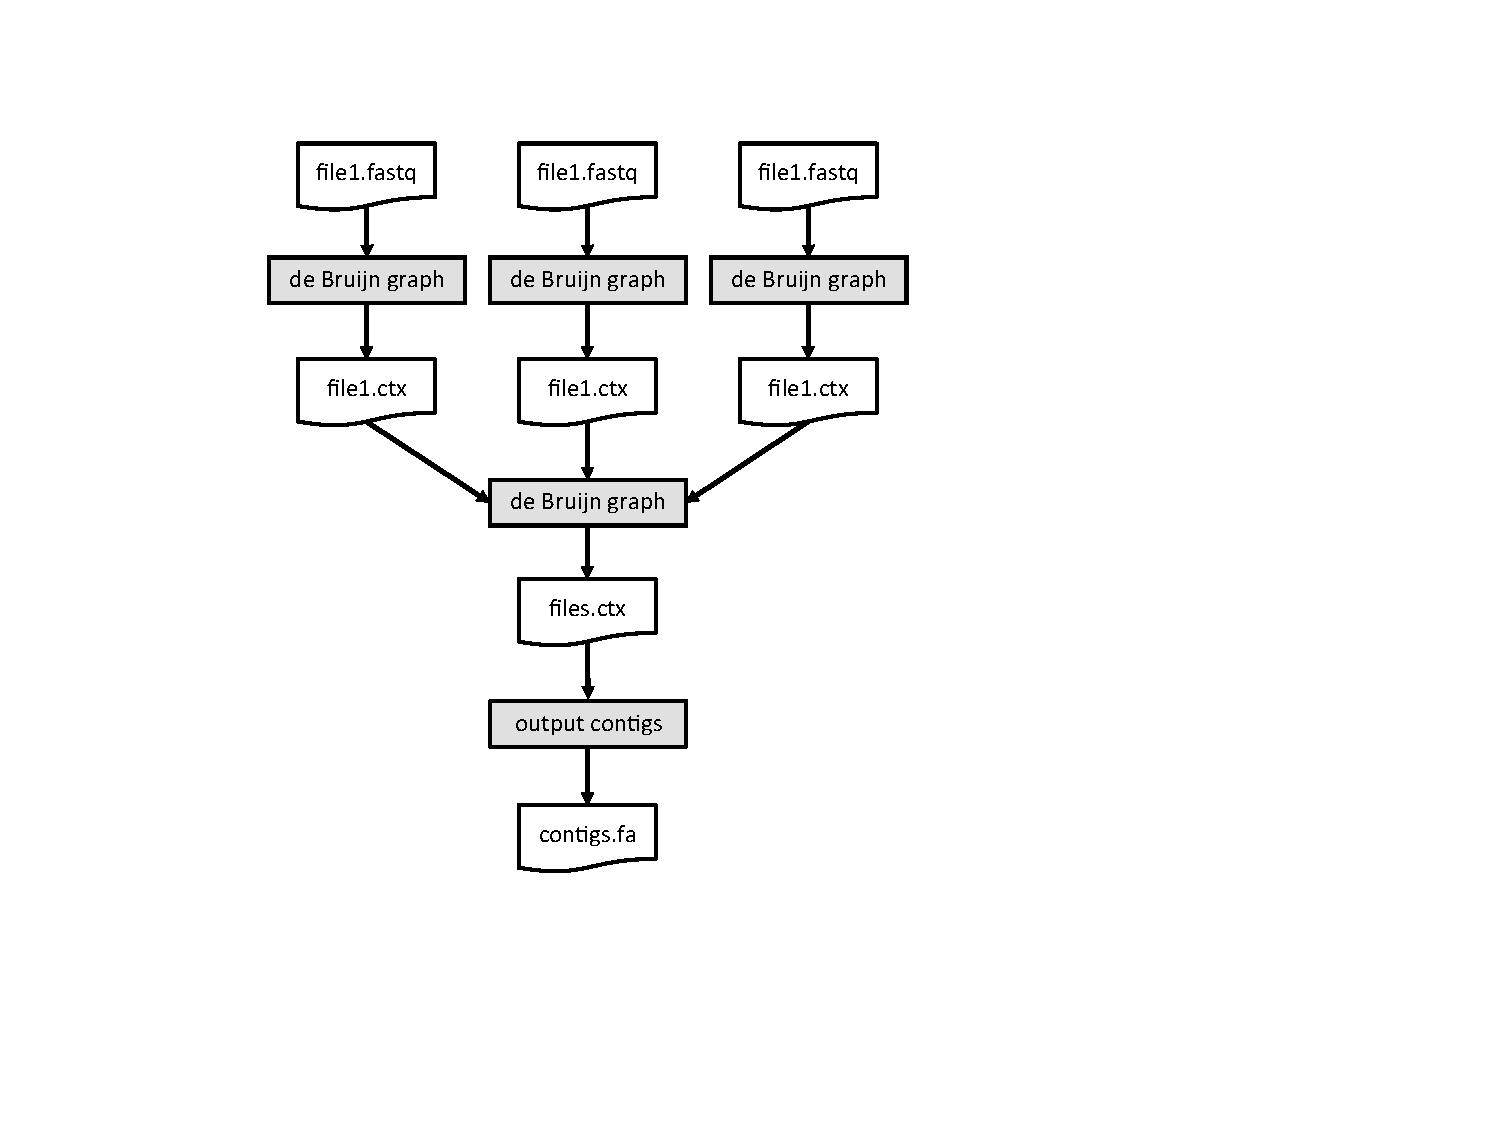
\includegraphics[width=8cm]{typicalprocess.pdf}
\caption[Typical scenario]{A typical scenario for running MetaCortex: individual files of reads are converted into de Bruijn graphs in parallel and CTX files are output. Then, the individual files are merged together into one single graph and contigs are output.} 
\label{fig:typicalprocess}
\end{figure}

%-------------------------------------------------------------------------
\subsection{Memory usage}

MetaCortex uses a hash table structure to store kmer information and the de Bruijn graph structure. You do not need to understand exactly how this structure works in order to use MetaCortex, but you do need to tell MetaCortex how much memory to set aside for the hash table. There are two parameters you need to specify - the hash table width, $n$, and the hash table height, $b$. The size of the hash table (the number of kmers that can be stored) is then given by $s = b \times 2^{n}$. This needs to be multiplied by the hash table entry size to find the total memory utilisation. The hash table entry size is 16 bytes for kmers of 31 nt or less, 24 bytes for kmers of 63 nt or less and 32 bytes for kmers of 95 nt or less. Table \ref{tab:examplememoryvalues} provides some examples to illustrate how the $n$ and $b$ parameters relate to hash table size and memory usage.

\begin{table}[htb]
\centering
\begin{tabular}{c c c c c c}
\hline
  &     & Capacity & Memory         & Memory          & Memory \\
n & b & (kmers)      & for k $\le$ 31 & for k $\le$ 63 & for k $\le$ 5  \\
\hline
15 & 100 & 3,276,800 & 50 Mb & 75 Mb & 100 Mb \\
20 & 100 & 104,857,600 & 1.6 Gb & 2.4 Gb & 3.2 Gb \\
25 & 100 & 3,355,443,200 & 51.2 Gb & 76.8 Gb & 102.4 Gb \\
\hline
\end{tabular}
\caption[Example values]{Some example values for $n$ and $b$ and how these relate to hash table capacity and memory usage.}
\label{tab:examplememoryvalues}
\end{table}

%-------------------------------------------------------------------------
\subsection{Cleaning options}

Cortex supports a number of cleaning options which are designed to remove kmers from the de Bruijn graph which are likely the result of errors. These options are included in MetaCortex too. However, it is recommended that in most metagenomic assembly situations, these are unused.

%=========================================================================
\section{Build and installation}

A decision needs to be made at compile-time on the largest k-mer size which you wish a given executable to support and this value may be either 31, 63, 95, 127, 160 or 192 nucleotides. Selecting this at compile-time allows for much more efficient use of memory during program execution. Often users will compile a number of different versions of the code, selecting at run-time the most appropriate one to use. The maximum kmer size may be specified as a parameter to the make command:
\vspace{6pt}
 \begin{verbatim}
$ make MAXK=31 metacortex
 \end{verbatim}
\vspace{-6pt}
 
\noindent{}This command should be executed in the directory containing the Makefile. When the build process completes, the executable may be found in the \verb|bin| directory as \verb|metacortex_kX| where $X$ is the maximum kmer size chosen. If building on Mac OS, it is necessary to specify an additional option:
\vspace{6pt}
 \begin{verbatim}
$ make MAXK=31 MAC=1 metacortex
 \end{verbatim}
\vspace{-6pt}

%=========================================================================
\section{Using MetaCortex}

\subsection{The one step process}

If the dataset you are dealing with is small enough and/or you have enough memory and time, you don't need to create intermediate CTX files and can go from FASTQ to contigs in one step:
\vspace{6pt}
\begin{verbatim}
$ echo "file1.fastq" > allfiles.txt
$ echo "file2.fastq" >> allfiles.txt
$ echo "file3.fastq" >> allfiles.txt
$ cortex_con_31 -k 31 -n 23 -b 65 -i allfiles.txt -t fastq -o all.ctx
                -f contigs.fa -g 100 -l log.txt
\end{verbatim}

\noindent Each time you run MetaCortex, you need to specify a `file of files', which is simply a plain text file that provides a list of the input files. In the above example, the first three lines create this file, then the second line invokes MetaCortex. The options have the following meanings:
\begin{itemize}
\item{the \verb=-k= option specifies the kmer size to be used for the de Bruijn graph.}
\item{the \verb=-n= and \verb=-b= options specify the hash table width and height to be used to store the de Bruijn graph.}
\item{the \verb=-i= option specifies the name of an input file of files. All files listed in this file will be merged to create a single graph.}
\item{the \verb=-t= option tells MetaCortex to expect FASTQ format files.}
\item{the \verb=-f= option specifies the name of the output contig file.}
\item{the \verb=-g= option tells MetaCortex to output only contigs of 100nt or more.}
\item{the \verb=-l= option specifies the name of an output log file.}
\end{itemize}

\subsection{Creating intermediate CTX files}

If you have many input files and you wish to process them separately, individual FASTQ files can be converted into CTX files (binary representations of the de Bruijn graph) using the following command:
\vspace{6pt}
\begin{verbatim}
$ echo "file1.fastq" > file1.txt
$ metacortex_k31 -k 31 -n 23 -b 65 -i file1.txt -t fastq -o file1.ctx
\end{verbatim}
\vspace{6pt}

\noindent  As before, the first line just creates a file of files. The new \verb=-o= option specifies the name of the binary output file.

\subsection{Merging CTX files and writing contigs}

Once you have a set of CTX files, these can be merged and contigs output. A typical command will look like the following:
\vspace{6pt}
\begin{verbatim}
$ echo "file1.ctx" > allfiles.txt
$ echo "file2.ctx" >> allfiles.txt
$ echo "file3.ctx" >> allfiles.txt
$ metacortex_k31 -k 31 -n 23 -b 65 -i allfiles.txt -t binary
                 -o all.ctx -f contigs.fa -g 100
\end{verbatim}
\vspace{6pt}
Again, we start by making a file of files - now containing all the CTX files. This time we specify `binary' for the -t option to tell Cortex to expect CTX files. 

\begin{thebibliography}{9}
\bibitem{iqbal2012}
Iqbal, Z, Caccamo, M, Turner, I, Flicek, P, McVean, G, De novo assembly and genotyping of variants using colored de Bruijn graphs, \emph{Nature Genetics}, 44:226-232, 2012.
\end{thebibliography}

\end{document}
